%Matteo Kumar - Leonhard Schatt
% Fortgeschrittenes Physikalisches Praktikum
 
\section{X-Rays}\label{sec:Q1}

X-rays are high energetic electromagnetic radiation with wavelengths between \SIrange{0.1}{10}{\angstrom} which corresponds to energies from \SIrange{1.24}{123.98}{\kilo\eV}~\cite{Bohm.2021}. However, for purposes of cristallography, usually wavelengths of \SIrange{0.5}{2.0}{\angstrom} are used~\cite{Schwarzenbach.2001}. X-rays can be generated in X-ray tubes. Such a tube is depicted in Fig. REF. In those, electrons are emitted, e.g.~by a glow wire, and accelerated by applying a high voltage (\SIrange{25}{100}{\kilo\V}). Due to hitting a metal anode, two different types of radiation are produced: Bremsstrahlung and the characteristic X-ray emission. The continous Bremsstrahlung occurs due to the scattering of the electrons at the metal atoms. The characteristic X-ray emission can be seen as discrete peaks in the emission spectrum. These correspond to the differences of the binding energies of different energy levels $\Delta E_i$ in the metal atoms. Photons of those $\Delta E_i$ can be emitted if the accelerated electrons knock out inner electrons of the metal atoms and electrons further out fall back on the free enery level~\cite{Bohm.2021}. An example of an X-ray emission spectrum can be seen in fig.~\ref{fig:xRaySpectrum}. \par 

\begin{figure}[ht]
    \centering
    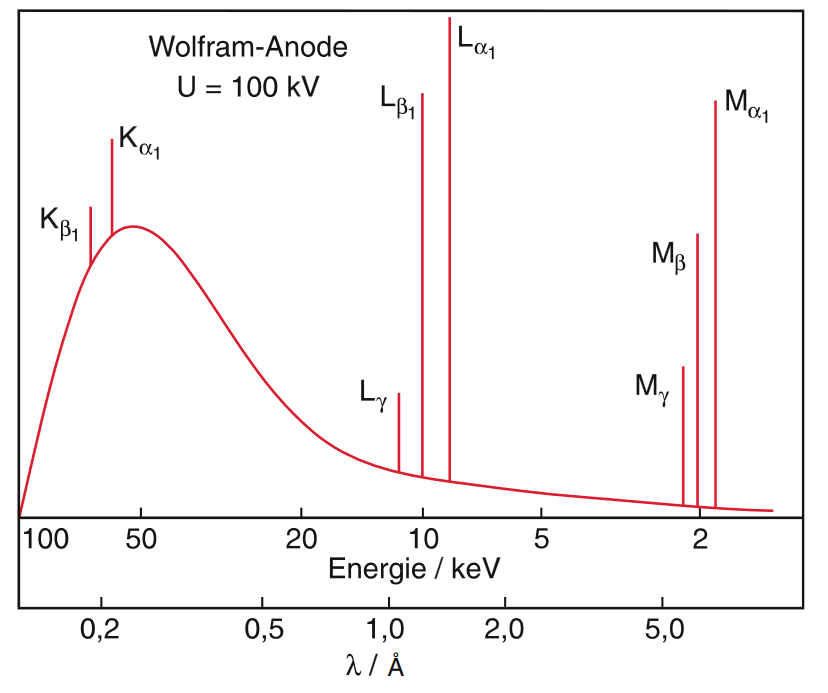
\includegraphics[width = 0.8\textwidth]{Bilder/Grundlagen/xraySpectrum.png}
    \caption{X-ray spectrum from a tungsten anode. The continious Bremsstrahlung can be seen aswell as the characteristic K, L and M lines. Figure from \cite{Demtroeder.2016}}
    \label{fig:xRaySpectrum}
\end{figure}

X-rays can also be produced in a synchrotron. Here, the change in acceleration in the bends of the synchrotron leads according to Maxwell's equations to the emission of radiation, the synchrotron radiation. Additionally, wigglers and undulators are used. They consist of a series of magnets, which lead the beam to undulate. Hereby, additional radiation in the mean direction of movement is generated. Wigglers produce a broader spectrum of radiation, undulators, in contrast, a line spectrum.



